\documentclass[
  captions=tableheading,
  bibliography=totoc, 
  titepage=firstiscover,
]{scrartcl}

\usepackage{blindtext} %neuer input

\usepackage{longtable} % Tabellen über mehrere Seiten

\usepackage[utf8]{inputenc} %neuer input

\usepackage{scrhack}

\usepackage[aux]{rerunfilecheck} %Warnung falls nochmal kompiliert werden muss

\usepackage{fontspec} %Fonteinstellungen

\recalctypearea{}

\usepackage[main=ngerman]{babel} %deutsche Spracheinstellung

\usepackage{ragged2e} %neuer input

\usepackage{amsmath, nccmath}

\usepackage{amssymb} %viele mathe Symbole

\usepackage{mathtools} %Erweiterungen für amsmath


\DeclarePairedDelimiter{\abs}{\lvert}{\rvert}
\DeclarePairedDelimiter{\norm}{\lVert}{\rVert}

\DeclarePairedDelimiter{\bra}{\langle}{\rvert}
\DeclarePairedDelimiter{\ket}{\lvert}{\rangle}

\DeclarePairedDelimiterX{\braket}[2]{\langle}{\rangle}{
#1 \delimsize| #2
}

\NewDocumentCommand \dif {m}
{
\mathinner{\symup{d} #1}
}


\usepackage[
  math-style=ISO,
  bold-style=ISO,
  sans-style=italic,
  nabla=upright,
  partial=upright,
  warnings-off={
    mathtools-colon,
    mathtools-overbracket,
  },
]{unicode-math}

\setmathfont{Latin Modern Math}
\setmathfont{XITS Math}[range={scr, bfscr}]
\setmathfont{XITS Math}[range={cal, bfcal}, StylisticSet=1]


\usepackage[
  locale=DE,
  separate-uncertainty=true,
  per-mode=reciprocal,
  output-decimal-marker={,},
]{siunitx}

\usepackage[autostyle]{csquotes} %richtige Anführungszeichen

\usepackage{xfrac}

\usepackage{float}

\floatplacement{figure}{htbp}

\floatplacement{table}{htbp}

\usepackage[ %floats innerhalb einer section halten
  section,   %floats innerhalb er section halten
  below,     %unterhalb der Section aber auf der selben Seite ist ok
]{placeins}

\usepackage[
  labelfont=bf,
  font=small,
  width=0.9\textwidth,
]{caption}

\usepackage{subcaption} %subfigure, subtable, subref

\usepackage{graphicx}

\usepackage{grffile}

\usepackage{booktabs}

\usepackage{microtype} %Verbesserungen am Schriftbild

\usepackage[
backend=biber,
]{biblatex}

\addbibresource{../lit.bib}

\usepackage[ %Hyperlinks im Dokument
  german,
  unicode,
  pdfusetitle,
  pdfcreator={},
  pdfproducer={},
]{hyperref}

\usepackage{bookmark}

\usepackage[shortcuts]{extdash}

%\usepackage{warpcol}

\usepackage{tikz}

\newcommand*\circled[1]{\tikz[baseline=(char.base)]{
            \node[shape=circle,draw,inner sep=2pt] (char) {#1};}}

\begin{document}
    \title{V602: Röntgenemission und -absorption}
    \author{  
    Paul Störbrock\\
    \texorpdfstring{\href{mailto:paul.stoerbrock@tu-dortmund.de}{paul.stoerbrock@tu-dortmund.de}}{}
    }
    \date{Abgabe: 19.05.2020\vspace{-4ex}}
\maketitle
    
\newpage
\tableofcontents
\newpage

\setcounter{page}{1}

\section{Ziel}

\section{Theorie}

\flushleft{Röntgenstrahlung\;}\justifying wird erzeugt, indem Elektronen von einer Glühkathode in einer evakuierten Rühre zu einer
Anode beschleunigt werden. Trifft ein beschleunigtes Elektron auf die Anode, wird das Elektronen abgebremst und verliert Energie. Die Abbremsung
erfolgt im Coulombfeld eines Atomkerns der Anode. Die verlorene Energie wird als Photon (Röntgenquant) abgestrahlt welches ein kontinuierliches 
Bremsspektrum erzeugt. Das Photon stellt die Röntgenstrahlung dar und besitzt die Charakteristik des Anodenmaterials. Das Bremsspektrum ist 
kontinuierlich, da das Elektron dessen gesamte kinetische Energie verlieren kann. 

\flushleft{Bei\;}\justifying der Wechselwirkung zwischen Elektron und Anode, wird das Anodenmaterial ionisiert. Das heißt, dass ein Elektron der
Anode auf höheres Energieniveau gebracht wird. Dies geschieht, indem das Elektron auf eine äußere Schale spring. Da nun eine Leerstelle auf der
inneren Bahn entstanden ist, kann ein Elektron von einer äußeren Schale auf die innere zurückfallen, also auf ein niedrigeres Energieniveau.
Demnach ist die Energiedifferenz $h\cdot\nu=E_m - E_n$ \cite{V602} der beiden Schalen $m,n$ die Energie des emittierten Röntgenquants. 
Das Charakteristische Spektrum besitzt scharfe Linien, welche als $K_{\alpha}, K_{\beta}, L_{\alpha}, L_{\beta}, M_{\alpha},...$ beschrieben werden. 
Die Buchstaben bezeichnen die Schale, wohingegen $\alpha$ oder $\beta$ die Zielschale des Elektrons bestimmt, welche dessen Energie abgestrahlt 
hat. 

\flushleft{Elektronen\;}\justifying auf einer höheren Schale erfahren eine geringere Anziehungskraft des Atomkerns, da Elektronen auf einer tieferen
Schale einen Teil der Kernladung abschirmen. Die Bindungsenergie zwischen einem Elektron auf der $n$-ten Schale kann dementsprechend mit der 
Formel \cite{V602}
\begin{align}
    E_n = -R_{\infty}\cdot z_{eff}^2 \cdot \frac{1}{n^2} \label{eq:1}
\end{align}
\flushleft{dargestellt\;}\justifying werden. Hierbei ist die Rydbergenergie $R_{\infty}=\SI{13.6}{\electronvolt}$ und 
\begin{align}
    z_{eff}=z-\sigma \label{eq:2}
\end{align}
\flushleft{die\;}\justifying effetive Kernladung, wobei z die Ornungszahl des Elements und $\sigma$ die Abschirmkonstante darstellt. 
Da neben der Coulomb Anziehung noch die Elektronen selbst durch den eigenen Spin und dem Bahndrehimpuls miteinander wechselwirken, sind die
charakteristischen Linien des Spektrums nicht scharf definiert. Die einzelnen Linien sind in eng beieinander liegenden Linien unterteilt. Diese 
Unterteilung heißt Feinstruktur, welche mit diesem Versuch hingegen nicht aufgelöst werden kann. 

\flushleft{Die\;}\justifying Absorption eines Materials ist energiebedingt und hängt von der Bindungsenergie ab. Wird die Bindungsenergie 
überschritten, wird das Elektron aus der jeweiligen Schale gelöst. Entweder wandert das Elektron auf eine energetisch höhere Schale (Compton-Effekt),
oder es wird ganz aus der Umlaufbahn des Atoms gestoßen (Photoeffekt). Das Absorptionsspektrum fällt mit zunehmender Energie ab und springt, wenn
die Bindungsenergie überschritten wird. Dieser Sprung im Graphen wird als Absorptionskante bezeichnet und als $K-, L-, M-,...$ Kante definiert. 
Die hier relevante Kante ist die $K-$Kante. Da das Absorptionsspektrum analog zum Emissionsspektrum nicht scharf definiert ist, muss die Bindungsenergie
eines Elektrons mit der Sommerfeldschen Feinstrukturformel \cite{V602} 
\begin{align}
    E_{n,j} &= -R_{infty} \left( z_{eff,1}^2 \cdot \frac{1}{n^2} + \alpha^2 z_{eff,2}^4 \cdot \frac{1}{n^3} \left( \frac{1}{j+\frac{1}{2}} - \frac{3}{4n} \right) \right) \label{eq:3}
\end{align}
\flushleft{bestimmt\;}\justifying werden. $R_{\infty}$ ist hier wieder die Rydbergenergie, $z_{eff}$ die Kernladungszahl, $\alpha$ die 
Sommerfeldsche Feinstrukturkonstante, $n$ die Hauptquantenzahl und $j$ der Gesamtdrehimpuls des jeweiligen Elektrons. Wird $z_{eff}=z-\sigma$
eingesetzt, lässt sich die Sommerfeldsche Feinstrukturformel nach der Abschirmkonstante $\sigma_{K,abs}$ umstellen. Daraus folgt: \cite{V602}
\begin{align}
    \sigma_{K,abs} &= z - \sqrt{\frac{E_K}{R_{\infty}} - \frac{\alpha^2 z^4}{4}} \label{eq:4}
\end{align}

\flushleft{Die\;}\justifying Energie des emittierten Photons 
\begin{align}
    E=\frac{hc}{\lambda e} \label{eq:5}
    \intertext{lässt sich mithilfe der Bragg'schen Bedingung
    }
    2d\sin(\theta) &= n\lambda \label{eq:6}
\end{align}
\flushleft{Bestimmen.\;}\justifying Die Bragg'sche Reflexion bezeichnet die Beugung der emittierten Röntgenstrahlung an einem Lithiumfluorid-Kristall (LiF-Kristall).
Dabei ist $d_{LiF}=\SI{201.4}{\pico\meter}$ \cite{V602} die Gitterkonstante des LiF-Kristalls, $\lambda$ die Wellenlänge der Strahlung, $\theta$
der Glanzwinkel und $n$ die Ordnungszahl. Das atomare Gitter des LiF-Kristalls beugt die Photonen und erzeugt im Glanzwinkel konstruktive 
Interferenz. 

\flushleft{Da\;}\justifying das Emissionsspektrum aufgrund der Sommerfeldschen Feinstruktur nicht eindeutig ist, sondern die Sprünge bzw. Peaks auf 
einem Intervall liegen, muss für die Breite der Linien das Auflösevermögen 
\begin{align}
    A = \frac{E_K}{\Delta E_{FWHM}} \label{eq:7}
\end{align}
bestimmt werden. $E_K$ ist hierbei die jeeweilige Kantenenergie und $\Delta E_{FWHM}$ ist die jeweilige Energie der Halbwertsbreite (HWB). Die HWB
beschreibt die Länge des Intervalls, in welcher sich die betrachtete Kante befindet. Im Falle von Kupfer werden die $K_{\alpha}$- und die
$K_{\beta}$-Linie betrachtet, welche in dem jeweiligen Intervall der $HWB_{K_{\alpha}}$ und $HWB_{K_{\beta}}$ liegen. Die halbe Amplitude der $K_{\alpha}$- 
bzw. $K_{\beta}$-Linie beschreibt Anfang und Ende der HWB. Die DiffAus der Differenz der Grenzen der HWB lässt sich die Energie der jeweiligen HWB
bestimmen, welche zum Auflösevermögen der Linie führt.

\section{Versuchsaufbau und -durchführung}

\flushleft{Benötigt\;}\justifying werden: \textit{Eine Kupfer-Röntgenröhre, ein LiF-Kristall, ein Geiger-Müller Zählrohr, ein Röntgengerät, ein 
Bromabsorber, ein Galliumabsorber, ein Rubidiumabsorber, ein Strontiumabsorber, ein Zinkabsorber und ein Zirkoniumabsorber.}

\flushleft{Das\;}\justifying Röntgengerät wird wie folgt aufgebaut:
\begin{figure}[H]
    \centering
    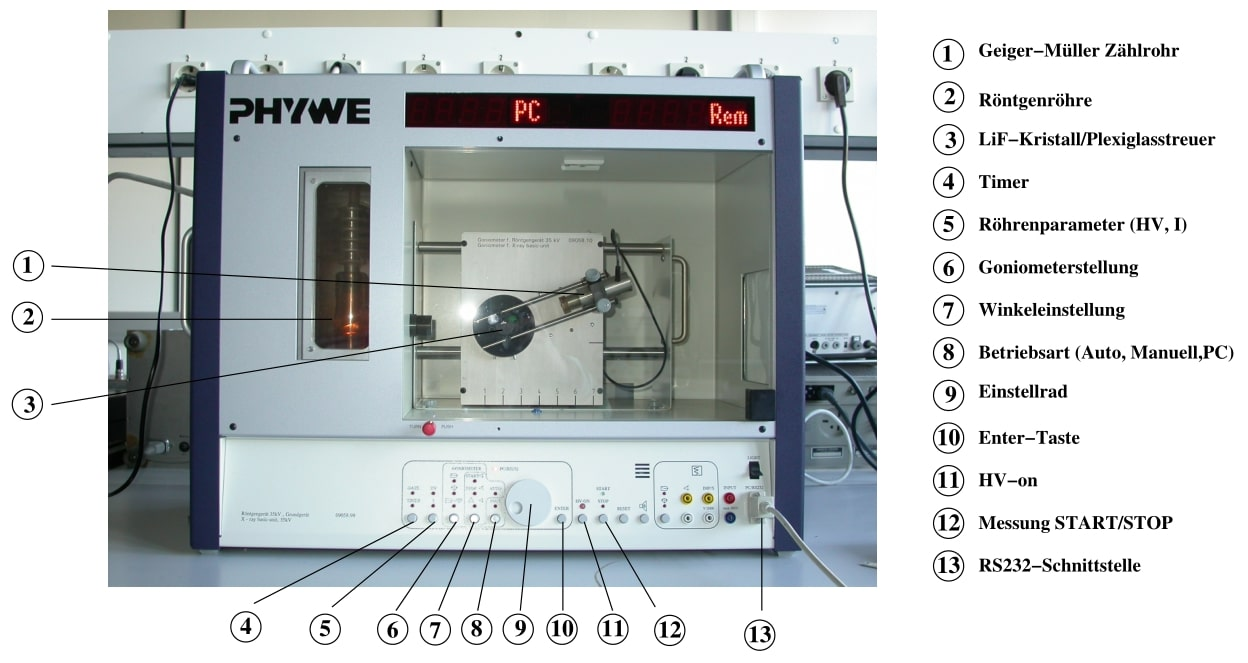
\includegraphics[width=\textwidth]{./images/Röntgenröhre.jpg}
    \caption{Aufbau der Röntgenröhre \cite{V602}}
\end{figure}
\flushleft{Zu\;}\justifying Beginn wird die Bragg Bedingung überprüft. Dazu wird der LiF-Kristall auf einen festen Winkel von $\theta=\SI{14}{\degree}$ gestellt und der
Winkelbereich des Geiger-Müller Zählrohrs variiert. Der Winkelbereich liegt zwischen $\SI{26}{\degree}\leq\alpha\leq\SI{30}{\degree}$ und wird in
$\SI{1}{\degree}$-Schritten bei einer Integrationszeit von $\Delta t=\SI{5}{\second}$ pro Winkel durchlaufen. 

\flushleft{Um\;}\justifying das Emissionsspektrum der Kupferröhre zu bestimmen wird diesmal das Geiger-Müller Zählrohr fixiert und der LiF-Kristall
variiert. Der Winkelbereich des LiF-Kristalls liegt hier zwischen $\SI{4}{\degree}\leq\alpha\leq\SI{26}{\degree}$ und wird ebensdalls in 
$\SI{1}{\degree}$-Schritten bei einer Integrationszeit von $\Delta t=\SI{5}{\second}$ pro Winkel durchlaufen.

\flushleft{Für\;}\justifying das Absorptionsspektrum der anderen Materialien wird der entsprechende Absorber angebracht. Hier wird der Winkelbereich
ebenfalls in $\SI{1}{\degree}$-Schritten durchlaufen, jedoch bei einer Integrationszeit von je $\Delta t=\SI{20}{\second}$ pro Winkel.
Die Winkelintervalle lauten wie folgt:\\
\begin{align*}
    &\SI{12.8}{\degree}\leq\theta_{\text{Brom}}\leq\SI{14.3}{\degree},\\ 
    &\SI{17}{\degree}\leq\theta_{\text{Gallium}}\leq\SI{19}{\degree},\\
    &\SI{11.2}{\degree}\leq\theta_{\text{Rubidium}}\leq\SI{12.5}{\degree},\\
    &\SI{10.5}{\degree}\leq\theta_{\text{Strontium}}\leq\SI{12}{\degree},\\
    &\SI{18}{\degree}\leq\theta_{\text{Zink}}\leq\SI{19.5}{\degree}\;\text{und}\\
    &\SI{9.5}{\degree}\leq\theta_{\text{Zirkonium}}\leq\SI{11}{\degree}.
\end{align*}


\section{Auswertung}

\flushleft{\;}\justifying

    \begin{figure}[H]
        \centering
        \includegraphics[width=\textwidth]{build/plotCu.pdf}
        \label{fig:}
    \end{figure}

\section{Diskussion}

\newpage
\section{Literatur}

\newpage
\section{Appendix}

    \input{table_Cu.tex}

    \begin{table}[H]
        \centering
        \caption{Bragg}
        \input{table_bragg.tex}
        \label{tab:2}
    \end{table}

    \begin{table}[H]
        \centering
        \caption{Brom}
        \input{table_brom.tex}
        \label{tab:3}
    \end{table}
    
    \begin{table}[H]
        \centering
        \caption{Gallium}
        \input{table_gallium.tex}
        \label{tab:4}
    \end{table}
    
    \begin{table}[H]
    \centering
        \begin{subtable}{.49\textwidth}
        \centering
        \caption{Rubidium}
        \input{table_rub.tex}
        \label{tab:5a}
        \end{subtable}    
        \begin{subtable}{.49\textwidth}
        \centering
        \caption{Strontium}
        \input{table_stron.tex}
        \label{tab:5b}
        \end{subtable}
        \begin{subtable}{.49\textwidth}
        \centering
        \caption{Zink}
        \input{table_zink.tex}
        \label{tab:5c}
        \end{subtable}    
        \begin{subtable}{.49\textwidth}
        \centering
        \caption{Zirkonium}
        \input{table_zirk.tex}
        \label{tab:5d}
        \end{subtable}
    \end{table}

\end{document}